% setting document languate
\documentclass[italian]{article}

% setting italian font encoding
\usepackage[utf8]{inputenc}
\usepackage[T1]{fontenc}
\usepackage{babel}
\usepackage{microtype}
\usepackage{ragged2e}
\usepackage{pgfplots}
\usepackage{makeidx}
\usepackage{sidecap}
\usepackage{graphicx}
\usepackage{subcaption}
\usepackage{float}
\graphicspath{ {./images/} }


\begin{document}
\justifying

\section*{Introduzione}
%Inserire introduzione

\section*{Tecnologie utilizzate}
Nella seguente sezione saranno elencate le tecnologie utilizzate per lo sviluppo del progetto. Alcune di esse, non facendo direttamente parte dello scopo del progetto, verranno passate in rassegna più rapidamente.
\subsection{LiDAR}
LiDAR, o Light Detection and Ranging, rappresenta uno strumeto di telerilevamento che determina la distanza di un oggetto o superfice tramite l'utilizzo di impulsi laser.\\
Il risultato di tale processo è una pointcloud.\\
\begin{figure}[H]
	\centering
	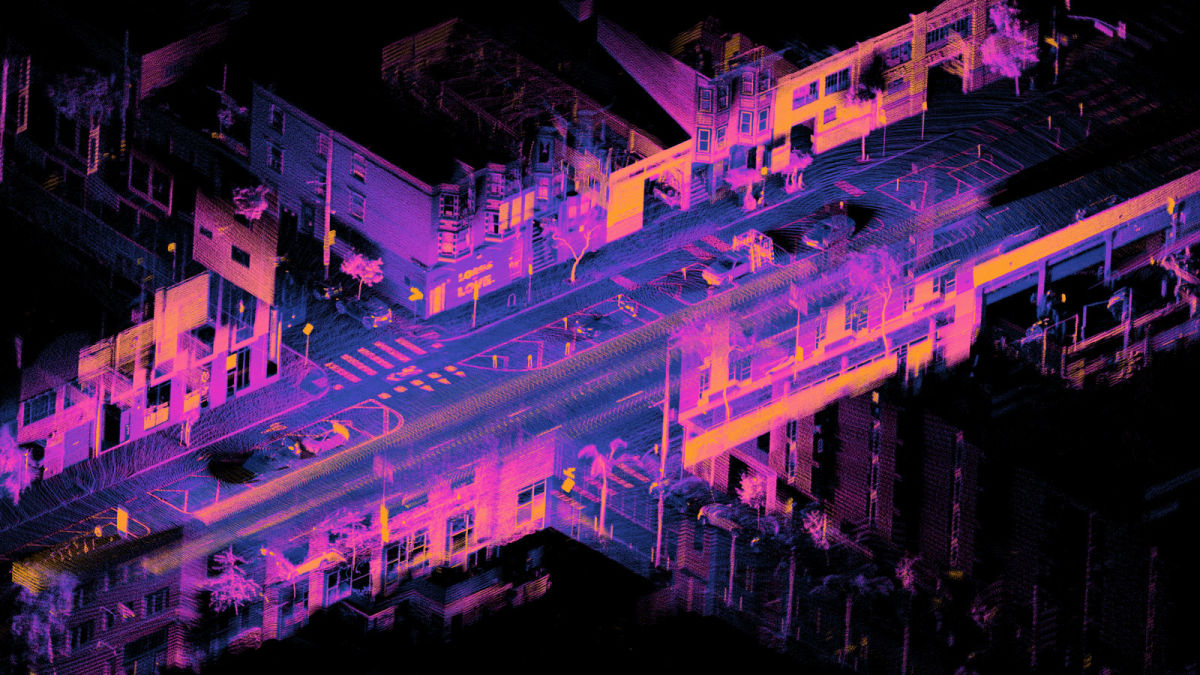
\includegraphics[width=0.9\textwidth]{LiDAR}
	\footnotesize
	\caption{Point cloud dettagliata di una strada ottenuta tramite LiDAR}
\end{figure}
\subsection{Datasets}
Affinché si avesse una generazione di pointcloud affidabile a partire dai dataset, è stato necessario l'utilizzo della tecnologia \textit{Arogverse} per l'acquisizione di scenari e modelli e di \textit{Blensor} per simulare scansioni LiDAR.
\subsubsection{Argoverse}
Argoverse è un dataset open-source di mappe, sviluppato dall'Università Carnegie Mellon e dal Georgia Institute of Tecnology negli Stati Uniti, il quale include metadati utili per lo sviluppo di sistemi a guida autonoma.\\
Tali dati sono stati raccolti a Miami e a Pittsburgh, due città caratterizzate da due comportamenti di guida differenti. Nel progetto è stata analizzata la mappa di un incrocio di Pittsburgh, incluso uno storico dei veicoli passanti (specificando per ciascuno ID, posizioni e velocità).\\
\begin{figure}[H]
	\centering
	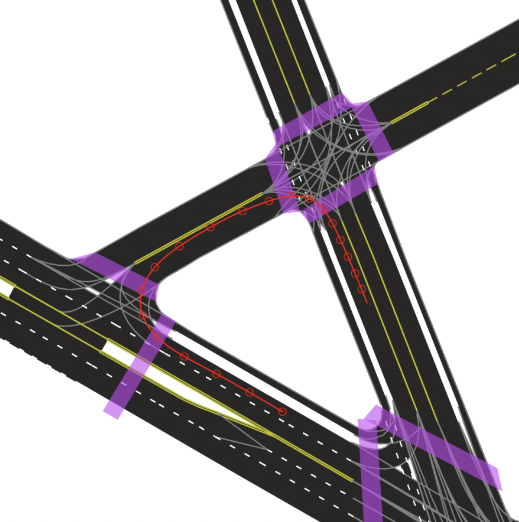
\includegraphics[width=0.9\textwidth]{Pittsburgh}
	\footnotesize
	\caption{Mappa di un incrocio di Pittsburgh}
\end{figure}\\
Nonostante le informazioni siano state raccolte attraverso veicoli con telecamere e sensori LiDAR, questi ultimi non influenzano assolutamente lo scopo del progetto.
\subsubsection{BlenSor}
BlenSor è un package dell'applicazione Blender che permette di simulare scansioni LiDAR. Sviluppato dall'Università di Salisburgo, ha come principale vantaggio quello di creare scenari che, nel caso della guida autonoma, nella realtà non sarebbero realizzabili o sarebbero troppo costosi da riprodurre (come per esempio una sitazione di incidente).\\
Nel nostro caso è risultato cruciale in quanto è stato possibile sfruttare algoritmi di norma presenti in sensori, senza possederli fisicamente.\\
\begin{figure}[H]
	\centering
	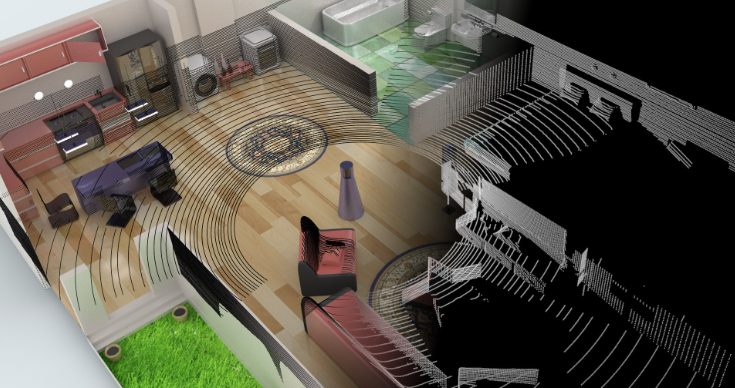
\includegraphics[width=0.9\textwidth]{Blensor}
	\footnotesize
	\caption{Scansione LiDAR simulata tramite Blensor}
\end{figure}\\
La simulazione tramite Blensor genera un file .csv per ogni istante e contiene le coordinate dei punti della pointcloud (senza rumore e filtrati, dove quest'ulitmo termina indica che vengono rimossi quei punti che rappresentano il terreno).
\subsection{Open3D}
Open3D è una libreria open-source che dispone di funzionalità grafiche per programmi Python e C++. Le principali features sono:
\begin{itemize}
	\item la possibilità di creare strutture dati 3D
	\item la presenza di algoritmi di data processing in 3D utilizzabili 
	\item lo sfruttamento della GPU per velocizzare operazioni più laboriose.
\end{itemize}
Per lo sviluppo del progetto sono stati sfruttati soprattutto i metodi di clusterizzazione delle pointcloud e di creazione delle bounding box a partire da cluster finiti, insieme alla visualizzazione grafica.
\subsubsection{Pointcloud}
La pointcloud è una struttura dati che rappresenta un insieme di punti nello spazio 3D. Viene istanziata tramite \textit{geometry.PointCloud()} e i punti (di coordinate (x,y,z)) vengono aggiunti come \textit{utlityVector3dVector(list)}\\
\begin{figure}[H]
	\centering
	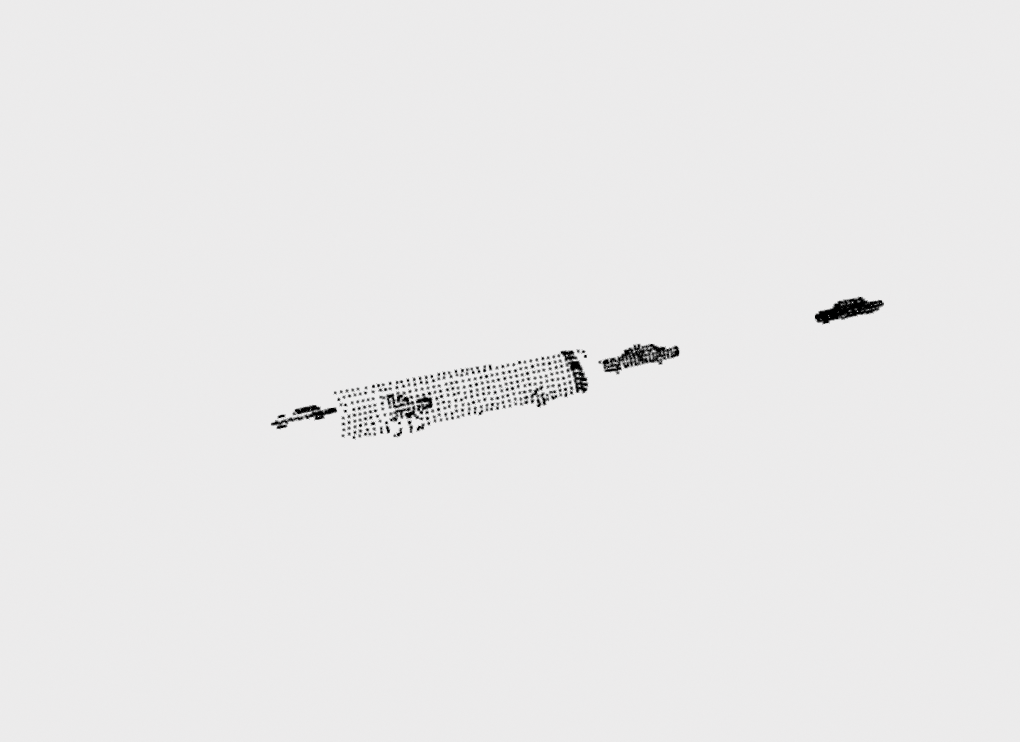
\includegraphics[width=0.7\textwidth]{Pointcloud}
	\footnotesize
	\caption{Esempio di pointcloud filtrata, senza noise e sottocampionata}
\end{figure}\\
\subsubsection*{Sottocampionamento}
Essendo il costo di campionamento delle pointcloud molto elevato a causa dell'alta densità di punti, è stato necessario sottocampionarle per avere una approssimazione accettabile in tempi ridotti. Attraverso \textit{pointcloud.voxeldownsample(size)}  viene sottocampionata la pointcloud attraverso cubi di lato \textit{size}. Questi ultimi dividono lo spazio 3D in griglie e se ciascun cubo presenta una serie di punti, ne verrà mantenuto uno solo.
\begin{figure}[H]
	\centering
	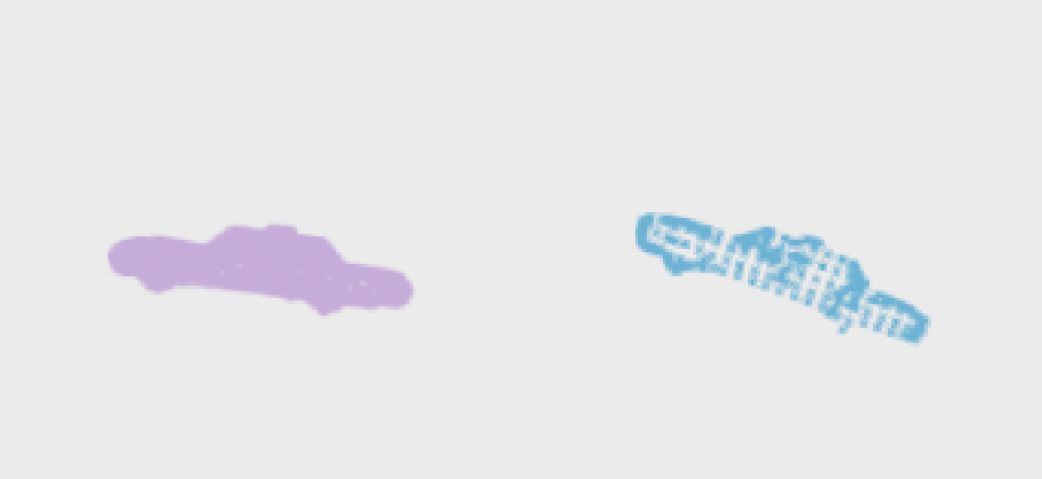
\includegraphics[width=0.7\textwidth]{Voxel}
	\footnotesize
	\caption{Esempio di processo di sottocampionamento della pointcloud}
\end{figure}
\subsubsection*{Clustering}
Open3D dispone di un algoritmo di clustering, \textit{pointcloud.cluster\_dbscan(eps, min\_points, print\_progress)}, che permette di clusterizzare i punti della pointcloud.\\
E' un metodo di raggruppamento di punti che si basa sulla distanza tra di essi e su un numero di punti minimo prestabilito che sta a indicare la presenza di un cluster.\\
Ovviamente questo metodo viene sfruttato solo in due situazioni nel progetto: per la prima creazione delle bounding box e per la clusterizzazione di punti esterni alle bounding box.
\subsubsection{Bounding Box}
Le Bounding Box sono rettangoli (o parallelepipedi in 3D) che racchiudono un insieme di punti della pointcloud.\\
Esistono tre categorie di bounding box:
\begin{itemize}
	\item Axis-Aligned Bounding Box (AABB): rappresenta una bounding box allineata con gli assi cartesiani. Dei tre è il più veloce da calcolare, ma può ricoprire più area del normale.
	\item Obiented Bounding Box (OBB): è una bounding box orientata in base alla forma della pointcloud. E' più accurata dell'AABB, ma richiede più tempo per essere calcolata.
	\item Minimum Bounding Box (MBB): individua la bounding box con la minima area che racchiude l'insieme di punti della pointcloud. Soprattutto in dimensioni superiori a due, richiede molto tempo per essere calcolata.
\end{itemize}
Nel nostro caso è stata utilizzata la bounding box di tipo OBB, in quanto la più accurata per lo scopo del progetto.
\begin{figure}[H]
	\centering
	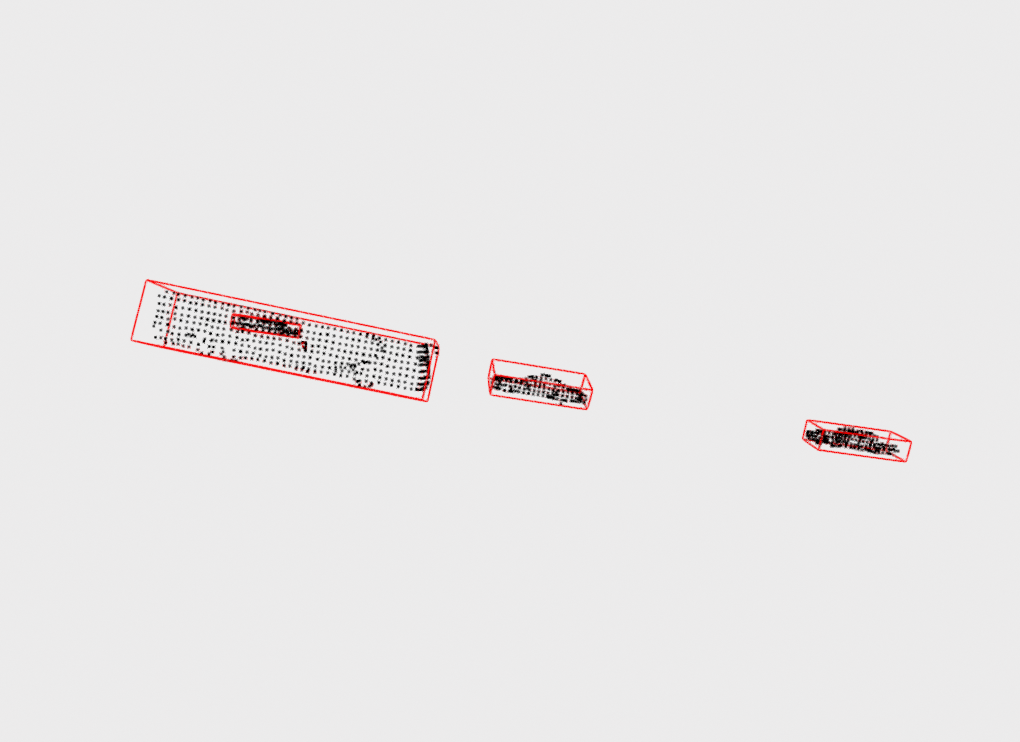
\includegraphics[width=0.7\textwidth]{bbox}
	\footnotesize
	\caption{Esempio di bounding box orientate}
\end{figure}\\
Open3D offre la possibilità di creare le bounding box a partire dalla pointcloud utilizzando il metodo \textit{pointcloud.get\_oriented\_bounding\_box)}, il quale ritorna un oggetto
\textit{geometry.OrientedBoundingBox}.\\
Le \textit{OrientedBoundingBox} possiedono l'attributo per assegnargli un colore, e cioè \textit{obb.color = [r,g,b]}.
\subsubsection*{Punti interni alla bounding box}
Siccome all'interno del programma sarà necessario aggiornare le bounding box nel modo più rapido possibile. La funzione\\ \textit{OrientedBoundingBox.get\_point\_indices\_within\_bounding\_box(pointcloud.points)} ha permesso di individuare gli indici dei punti interni alla bounding box presa in analisi dal programma in quell'istante di tempo, da cui poi creare il nuovo cluster e aggiornarla.\\ 
Essenzialmente analizza un insieme punti della pointcloud dati come argomento alla funzione (in questo caso \textit{pointcloud.points}) e ritorna un array di indici relativi ai punti di quest'ultima. Un punto viene considerato interno alla bounding box se, proiettato sui tre assi, risulta compreso tra i valori minimi e massimi determinati attraverso l'attributo \textit{extent} della OBB.\\
Questo metodo è ottimizzato per pointcloud di grandi dimensioni e garantisce un'ottima accuratezza nell'individuare i punti.
\subsubsection*{Centro, estensione e orientazione della bounding box}
L'oggetto \textit{geometry.OrientedBoundingBox} dispone di tre attributi fondamentali:
\begin{itemize}
	\item center: rappresenta il centroide della bounding box.
	\item extent: rappresenta l'estensione della bounding box. Sono tre valori che rappresentano l'altezza, la larghezza e la profondità della bounding box e rispettano l'orientamento di quest'ultima.
	\item R: rappresenta una matrice 3x3 che definisce l'orientamento della bounding box nello spazio tridimensionale.
\end{itemize}
Le seguenti informazioni hanno permesso di espandere la bounding box e includere nuovi punti alla porzione di pointcloud che si sta prendendo in analisi.
\begin{figure}[H]
	\centering
	\begin{subfigure}{0.45\textwidth}
		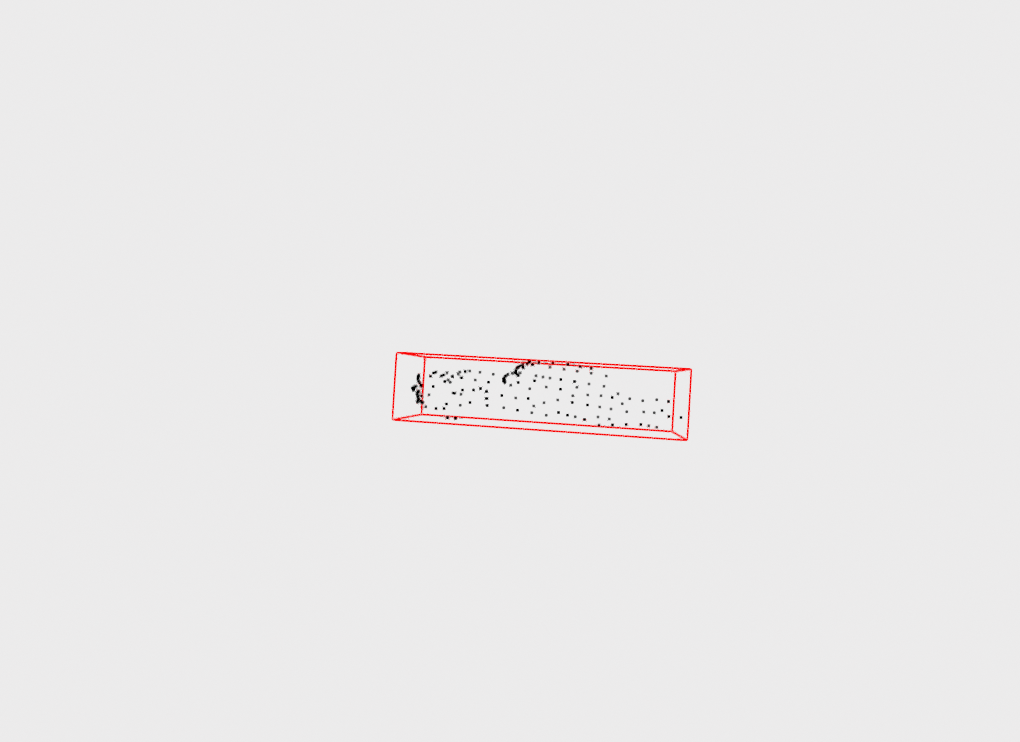
\includegraphics[width=\textwidth]{notExpandedBox}
	\end{subfigure}
	\begin{subfigure}{0.45\textwidth}
		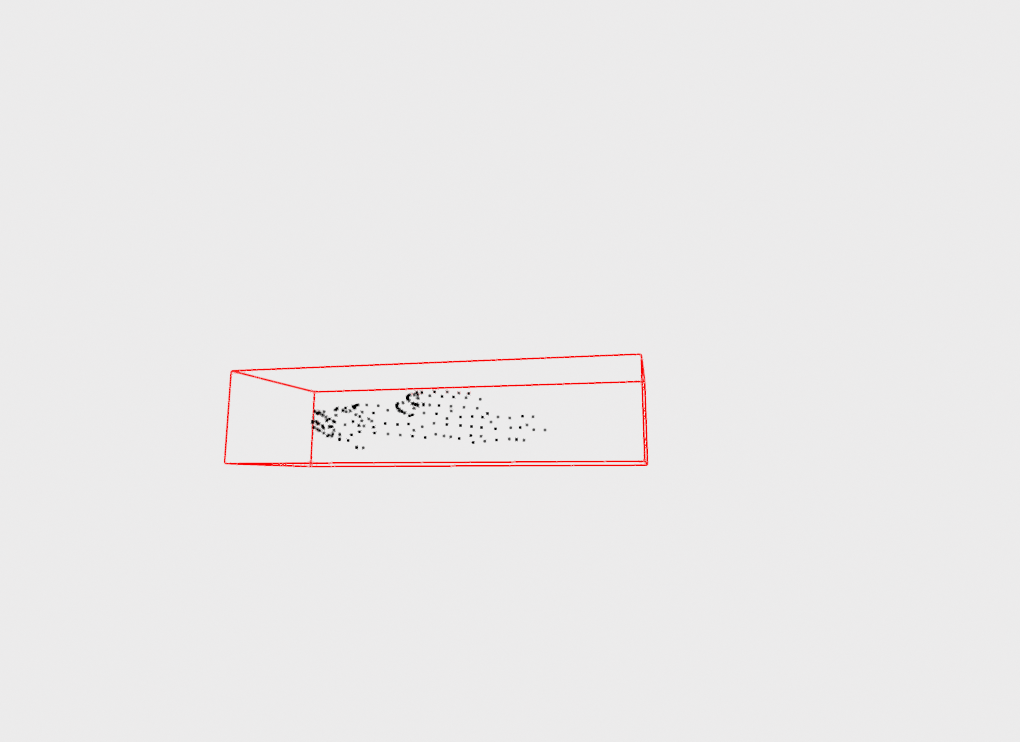
\includegraphics[width=\textwidth]{expandedBox}
	\end{subfigure}
	\footnotesize
	\caption{Espansione della bounding box}
\end{figure}

\subsubsection{Sfera}
Uno dei due metodi di clusterizzazione implementati prevede la creazione di una sfera a partire dai dati forniti da una bounding box. Open3D permette di istanziare un oggetto \textit{open3d.geometry.TriangleMesh} che crea e manipola geometrie 3D a mesh triangolari. Una mesh triangolare è un tipo di mesh poligonale in cui la superficie di un oggetto 3D è composta da facce triangolari.\\
Il metodo \textit{open3d.geometry.TriangleMesh.create\_sphere(radius)} crea una sfera di raggio \textit{radius} centrata nel centroide della bounding box attraverso il metodo \textit{translate(translation)}.\\
Essendo una sfera colorata, impedisce la visualizzazione dei punti interni: è stato necessario quindi trasformarla in un wireframe. Istanziando un oggetto\\ \textit{open3d.geometry.LineSet.create\_from\_triangle\_mesh(mesh)}, quest'ultimo permette di estrarre dalla mesh della sfera i lati dei triangoli che la compongono, così da permettere la visualizzazione dei punti interni.\\
\begin{figure}[H]
	\centering
	\begin{subfigure}{0.45\textwidth}
		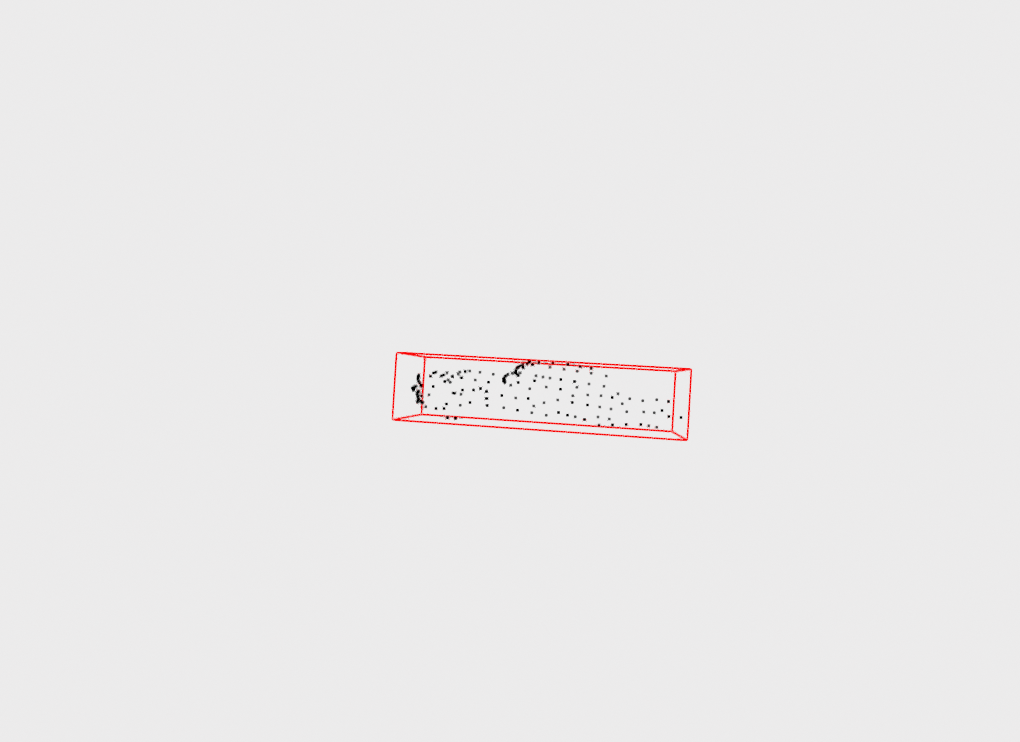
\includegraphics[width=\textwidth]{notExpandedBox}
	\end{subfigure}
	\begin{subfigure}{0.45\textwidth}
		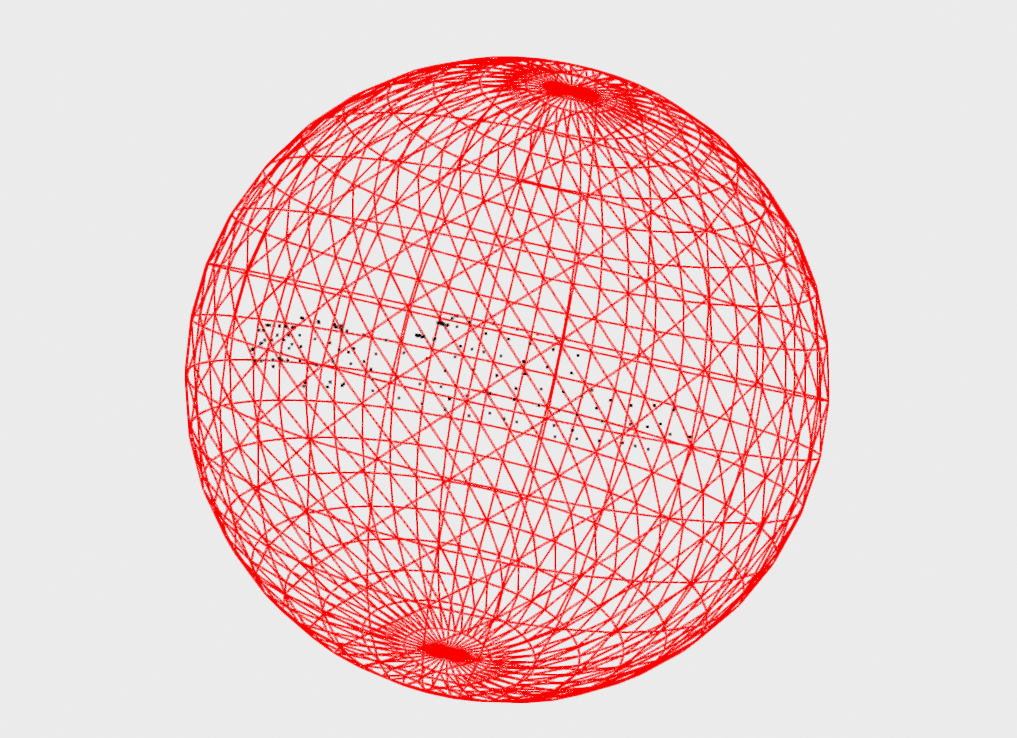
\includegraphics[width=\textwidth]{Sphere}
	\end{subfigure}
	\footnotesize
	\caption{Creazione di una sfera a partire dalla bounding box}
\end{figure}
\subsubsection{Draw}
Open3D offre la possibilità di visualizzare tramite interfaccia grafica le pointcloud e le bounding box attraverso il metodo \textit{open3d.visualization.draw()}, che permette anche di navigare liberamente all'interno della finestra, di zoomare e/o ruotare gli oggetti.\\
Sono presenti inoltre parametri che permettono una visualizzazione più personalizzata come
\begin{itemize}
	\item mostrare o nascondere piani arbitrari oppure
	\item mostrare o nascondere gli assi di riferimento
\end{itemize}

\begin{figure}[H]
	\centering
	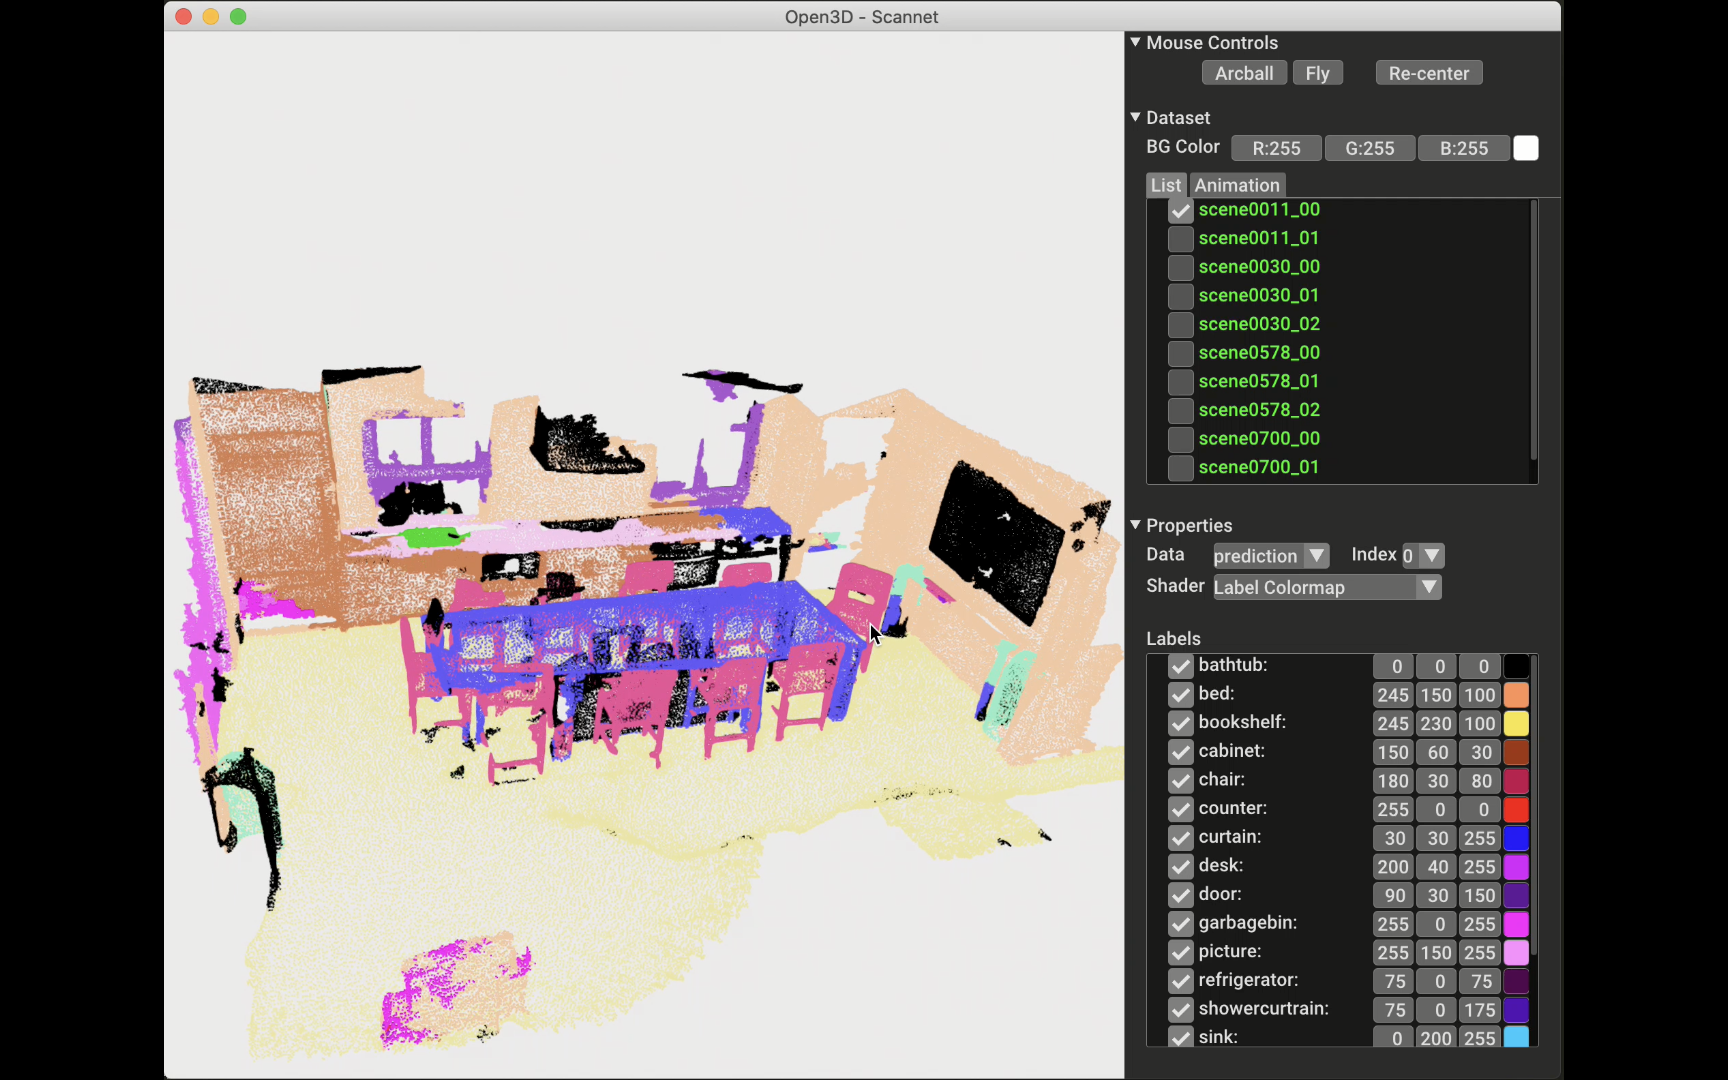
\includegraphics[width=0.7\textwidth]{o3dInterface}
	\footnotesize
	\caption{Esempio di interfaccia grafica di Open3D, con tabella di menu a destra}
\end{figure}\\


Le rappresentazioni tramite interfaccia grafica sono state sfruttate soprattutto per mostrare i passaggi che effettua il programma.

\section*{Alogirtmi}
Nella seguente sezione verranno trattati i principali algoritmi implementati per il progetto.
\subsection{Clustering}
Il clustering è un metodo di Unsupervised Learning che raggruppa un insieme di oggetti in classi simili. Tali classi possono essere di tipo morfologico, cromatico o basata sulle densità degli oggetti.\\
E' usato principalmente nell'esplorazione dei dati per ridurne la complessità di ricerca, per raggrupparli in maniera efficiente oppure per comprimerli.\\
L'algoritmo di clustering clustering implementato nel progetto è il DBSCAN.
\subsubsection{DBSCAN}
L'algoritmo DBSCAN divide i punti della pointcloud in batch o gruppi in base, in questo caso, alla densità.\\
Prima di descrivere l'argoritmo nel dettaglio, è necessario definire le seguenti terminologie:
\begin{itemize}
	\item Core point: un punto è un core point se ha almeno un numero minimo di punti vicini, il cui valore è chiamato \textit{minPts}, entro una certa distanza, chiamata \textit{epsilon} o \textit{eps}.
	\item Border point: un punto è un border point se non è un core point, ma è raggiungibile da un core point.
	\item Noise point: un punto è un noise point se non è nè un core point nè un border point.
\end{itemize}
\begin{figure}[H]
	\centering
	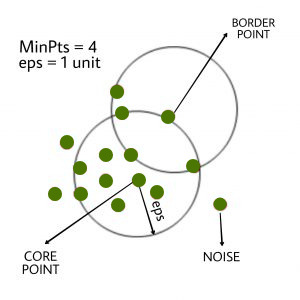
\includegraphics[width=0.5\textwidth]{clustering}
	\footnotesize
	\caption{Illustrazione di core point, border point e noise point}
\end{figure}\\
I passi principali dell'algoritmo sono:
\begin{itemize}
	\item individua i core points.
	\item per ogni core point che non è stato assegnato a un cluster, ne crea uno nuovo, aggiungendo tutti i punti raggiungibili.
	\item cerca ricorsivamente i punti \textit{density-connected} e li aggiunge allo stesso cluster come core points. Per \textit{density-connected} si intende che due punti sono collegati se esiste un core point che li collega.		Quindi se un punto \textit{b} è raggiungibile da un punto \textit{a} (e quindi che si trova a una distanza massima \textit{eps}), e un punto \textit{c} è raggiungibile da \textit{b}, allora \textit{c} è raggiungibile da \textit{a}.
	\item ripete i passi precedenti fino a quando tutti i punti sono assegnati a un cluster. Quelli che non appartengono neanche a uno, sono considerati noise points.
\end{itemize}
\begin{figure}[H]
	\centering
	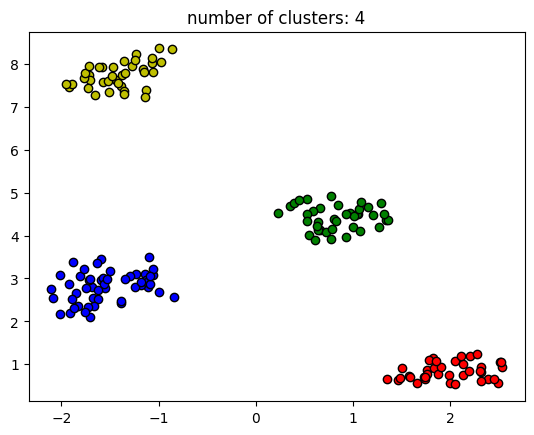
\includegraphics[width=0.7\textwidth]{dbscan}
	\footnotesize
	\caption{Clustering di una pointcloud tramite DBSCAN}	
\end{figure}\\
Rappresenta un algoritmo molto resistente a noise e può individuare cluster di forma arbitraria. La complessità dell'algoritmo è quadratica ($O(n^2)$)\\
Come accennato in precedenza, nel caso del progetto viene utilizzato solo per clusterizzare le pointcloud all'avvio del programma e ogni volta che ci sono nuove pointcloud da analizzare e non hanno una bounding box associata.
\subsubsection{DBSCAN personalizzato}
L'algoritmo di DBSCAN personalizzato, rispetto a quello originale, prende in considerazione dei punti già clusterizzati come punto di partenza e che completasse la creazione di un solo cluster per volta.\\
Quindi, partendo da delle bounding box già inizializzate (che vengono distinte dal colore verde) e dalla pointcloud di uno scan successivo, l'algoritmo compie i seguenti passaggi:
\begin{itemize}
	\item data la bounding box, individua gli indici dei punti interni sfruttando la funzione \textit{get\_point\_indices\_within\_bounding\_box()} che chiameremo \textbf{punti core}.
	\item a seconda del metodo di clusterizzazione scelto espande/ trasforma la bounding box in due modi differenti.
		\begin{itemize}
			\item dbscan\_expand\_bbox: espande la bounding box creandone una nova aumentata di una percentuale prestabilita e riutilizza la funzione citata precedentemente per ottenere gli indici dei nuovi punti.
			\item dbscan\_sphere\_bound: genera una sfera con centro nel centroide della bounding box e di raggio pari alla dimensione maggiore della bounding box per un fattore di espansione dato in input, diviso due 					per indicare il raggio. Successivamente individua gli indici dei punti interni alla sfera.
		\end{itemize}
	\item una volta deifiniti questi due set di indici, istanzia un array di label delle stesse dimensioni del numero di indici dei punti generati dal file \textit{dbscan\_expand\_bbox} o \textit{dbscan\_sphere\_bound} e vengono settati a -1, per indicare che sono noise. Successivamente setta a 1 tutti quegli indici che sono presenti anche nei \textbf{punti core}.
	\item a questo punto viene applicato l'effettivo algoritmo dbscan, con la differenza che parte dai punti che hanno label 1 (cioè che sono già considerati appartenenti a un cluster) e cerca ricorsivamente i punti vicini e clusterizza quelli che hanno label -1.
	\item la lista di label viene sfruttata per creare un solo cluster, dal quale si genera la bounding box aggiornata e sarà colorata di rosso.
	\item se in uno scan successivo il numero minimo di punti per formare un cluster è troppo basso, l'oggetto non viene più seguito e viene cancellata la bounding box associata.
\end{itemize}
Con questo approccio, si pressuppone che si possa clusterizzare le pointcloud in maniera più efficace rispetto all'algoritmo implementato da open3d in quanto si parte con luster già avviati.\\
\subsection{Intersezione di bounding box}
Avendo la possibilità di clusterizzare pointcloud esterne alle bounding box, può capitare che in un istante precedente si abbia una bounding box che contiene solo parte di un oggetto (in quanto il veicolo sta ancora entrando nel range dei sensori) e che in un istante successivo si abbia una nuova bounding box che contiene la parte restante, o l'oggetto completo, ma che comunque si sovrappone alla precedente.\\
\begin{figure}[H]
	\centering
	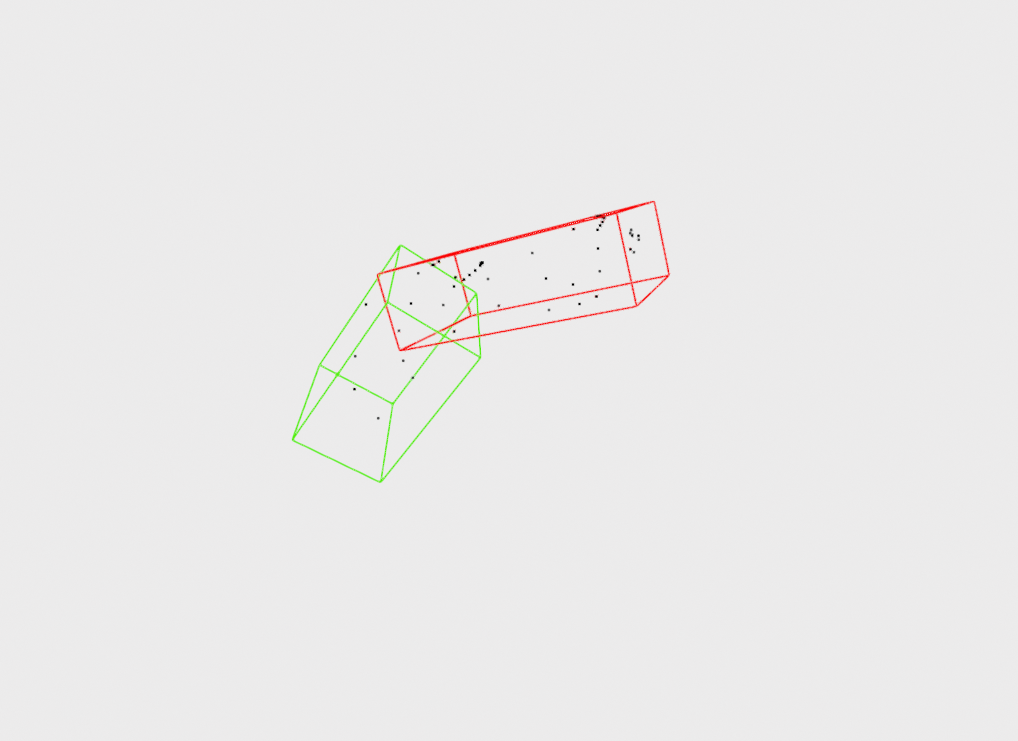
\includegraphics[width=0.7\textwidth]{Overlapping}
	\footnotesize
	\caption{Situazione di overlapping tra bounding box}
\end{figure}\\
Per ovviare a ciò è risultato necessario implementare un algoritmo che confronta le bounding box a coppie. Partendo dagli 8 vertici di ciascuna bounding box, si controlla se i vertici di una sono contenuti, anche in parte, all'interno dell'altra. Questa operazione è possibile verificando la sovrapposizione(ovrelap) minima e massima di ciascun asse.\\
Dati come assi di riferimento i tre cartesiani:
\begin{itemize}
	\item l'overlap minimo viene calcolato tramite valore massimo di ciascuna delle coordinate interessate delle due bounding box prese in analisi che hanno valore minimo.
	\item l'overlap massimo viene calcolato tramite valore minimo di ciascuna delle coordinate interessate delle due bounding box prese in analisi che hanno valore massimo.
\end{itemize}
Se gli overlap massimi di ciascun asse sono maggiori degli overlap minimi, allora siginfica che le bounding box si sovrappongono e quindi viene rimossa quella che ha volume minore. Questo valore è ottenuto dalla funzione \textit{get\_volume()} che calcola il volume della bounding box come prodotto delle lunghezze dei tre lati.\\

\section*{Progetto}
Lo scopo del progetto consiste nell'aggiornare le bounding box generate inizialmente dall'algoritmo della repository \textit{blensor\_analysis} in modo da ottimizzare la clusterizzazione delle pointcloud interne alle bounding box. A seconda delle necessità, la clusterizzazione delle pointcloud in istanti successivi viene effettuata o all'interno di bounding box espanse oppure all'interno di sfere.\\
I principali parametri che ne determineranno le prestazioni sono il tempo di esecuzione e la precisione delle bounding box.\\ 
Il programma è strutturato nella seguente maniera:
\begin{itemize}
	\item importazione della prima scansione, generazione delle pointcloud e creazione delle prime bounding box
	\item aggiornamento delle bounding box a ogni scansione successiva e visualizzazione grafica di ogni passaggio
\end{itemize}
\subsection{Hardware e librerie utilizzati}
Le principali librerie e il package utilizzato per lo sviluppo dell'applicativo python sono:
\begin{itemize}
	\item blensor\_analysis per la generazione delle prime bounding box e per la creazione delle pointcloud utili agli istanti successivi
	\item open3D
	\item numpy per la gestione di array
\end{itemize}
Come hardware invece è stato utilizzato un computer con processore i5-10600k e 16GB di RAM. Come IDE è stato utilizzata neovim.
\subsection{Note sul progetto}
Come detto in precedenza, si sta analizzando un incrocio di Pittsburgh, nel quale sono stati posizionati 5 sensori ad altezza 2.5 metri da terra. La frequenza di scansione, in base alla velocità media dei veicoli, è di 10Hz.
\begin{figure}[H]
	\centering
	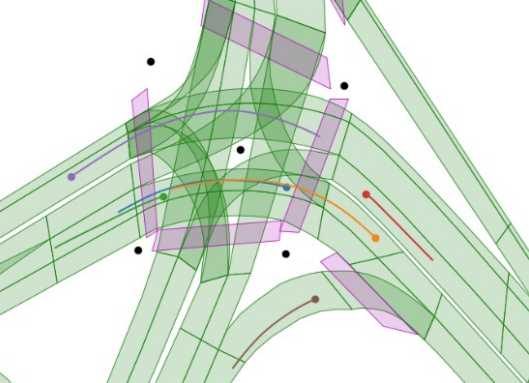
\includegraphics[width=0.7\textwidth]{junction_sensors}
	\footnotesize
	\caption{Incorcio di Pittsburgh con i 5 sensori (in nero)}
\end{figure}\\
\subsection{importazione della prima scansione, generazione delle pointcloud e creazione delle prime bounding box}
In questa fase iniziale del progetto viene sfruttato il modulo \textit{blensoranalysis} che invoca i principali metodi della repository \textit{blensor\_analysis} per importare la pointcloud iniziale dal rispettivo file \textit{.csv}, generando anche i cluster e le bounding box, e rendendendoli visibili tramite finestra generata da Open3D.\\
In questo caso è stato deciso che le pointcloud venissero preventivamente filtrate, rimuovendo gli scan del terreno, e senza rumore, in quanto non fanno parte dello scopo del progetto.\\
\subsection{aggiornamento delle bounding box a ogni scansione successiva}
A questo punto vengono coinvolti i moduli \textit{bbtracking.py}, \textit{dbscan\_expand\_bbox.py} (o \textit{dbscan\_sphere\_bound.py}) e \textit{blensoranalysis} per l'aggiornamento delle bounding box.\\
In \textit{bbtracking.py} vengono aggiornate le bounding box di partenza considerando la pointcloud dello scan successivo. Questi dati, insieme alle pointcloud degli scan successivi, sono ottentuti grazie ai metodi del modulo \textit{blensoranalysis}. Se durante il procedimento di aggiornamento delle bounding box una di esse contiene una porzione di pointcloud che non è abbastanza grande, allora viene eliminata e considerata noise.\\
Se durante l'aggiornamento delle bounding box in un determinato istante si presenta una nuova pointcloud che non è associata a nessuna bounding box, allora verrà applicato il clustering di Open3d che genera una nuova bounding box alla quale verrà associato il colore verde. Se quest'ultima si sovrappone a una bounding box già presente, allora viene rimossa quella con volume minore.\\
A livello visivo, verranno mostrate le seguenti situazioni:
\begin{itemize}
	\item quando si hanno le bounding box dell'iterazione corrente le bounding box dello scan succesivo.
	\item quando si effettua l'operazione di espasione delle bounding box generando una buonding box ingrandita oppure una sfera.
	\item quando si hanno nuovi cluster e quindi nuove bounding box.
	\item quando ogni pointcloud è stata correttamente clusterizzata e le bounding box sono state aggiornate corettamente.
\end{itemize}

\section*{Esiti}
Avendo preso in anlisi una situazione ideale di traffico, e cioè che i veicoli sono abbastanza distanziati da non causare errori nella creazione dei punti core e che non variano la direzione bruscamente, si ha che le bounding box aggiornate sono molto precise e che il tempo di esecuzione è sufficientemente basso.\\
\subsection{Tempo di esecuzione}
Per poter avere una stima temporale del programma, è stata sfruttata la libreria \textit{time} di Python.\\
Il tempo di esecuzione è stato calcolato tenendo conto del tempo di caricamento della pointcloud e del tempo di esecuzione dell'algoritmo di clusterizzazione e di aggiornamento delle bounding box.\\
Per avere una metodo di paragone, è stato calcolato anche il tempo di esecuzione del programma che ha eseguito soltanto la clusterizzazione tramite Open3D.\\
Per ogni esecuzione sono stati analizzati 5 scan eseguiti da 1 a 5 sensori. Attraverso questi 5 scan è stato calcolto il tempo di esecuzione medio\\
Ovviamente, maggiore è il numero di sensori e maggiore sarà il tempo di esecuzione richiesto.\\
\begin{tikzpicture}
	\begin{axis}[
		title={Tempo di esecuzione del programma},
		xlabel={Numero di sensori},
		ylabel={Tempo di esecuzione (s)},
		xmin=1, xmax=5,
		ymin=0, ymax=190,
		xtick={1,2,3,4,5},
		ytick={0,20,40,60,80,100,120,140,160,180, 200},
		legend pos=north west,
		ymajorgrids=true,
		grid style=dashed,
		width=12cm,
		height=8cm,
		axis xshift= -1 cm,
		axis yshift= -1 cm
		font=\footnotesize
	]
	\addplot[
		color=blue,
		mark=square,
		]
		coordinates {
			(1,5.521)(2,20.405)(3,47.537)(4,95.903)(5,184.660)
		};
	\addplot[
		color=red,
		mark=square,
		]
		coordinates {
			(1,4.999)(2,19.495)(3,51.556)(4,109.450)(5,181.146)
		};
	\addplot[
		color=green,
		mark=square,
		]
		coordinates {
			(1,5.535)(2,21.219)(3,53.987)(4,104.081)(5,178.993)
		};
	\legend{Espanione Bounding Box, Clusterizzazione Open3D, Sfera}
	\end{axis}
\end{tikzpicture}\\
Dal grafico si evince che per i primi due sensori il tempo di esecuzione varia molto poco tra i tre metodi, mentre per i sensori successivi si ha una differenza un po' più marcata.\\
Infatti i metodi di clusterizzazione personlaizzata implementati dal programma mostrano un lieve miglioramento nei tempi di esecuzione soprattutto quando si arriva ad avere un numero di sensori superiore a 3.\\ 
Ciò che può saltare all'occhio è come, raggiunti i 5 sensori, il tempo di esecuzione del programma che esegue l'espansione delle bounding box sia il più lungo di tutti. Questo può essere dovuto al fatto che durante la creazione delle bounding box espanse siano stati coinvolti un gran numero di punti, che hanno portato quindi a un rallentamento del programma.\\
In generale però si può notare che avere delle prime forme di cluster definite dai punti interni delle bounding box di partenza ha portato a un miglioramento dei tempi di esecuzione in quanto i punti da clusterizzare sono molto meno.
\subsection{precisione delle bounding box}
Considerando una situazione in cui la frenquenza di aggiornamento dei sensori è tale da far variare di poco lo spostamento degli oggeti, non si noterà grande differenza tra i due metodi di clusterizzazione personalizzata.\\
Questa considerazione può essere più impattante nelle situazioni in cui i veicoli si muovono in modo brusco e in direzioni diverse, in quanto il metodo di espansione delle bounding box potrebbe non essere in grado di reagire adeguatamente. Se si ha invece una sfera come riferimento è più probabile che includa eventuali punti in maniera più corretta.\\

\section*{Conclusioni}
Il progetto ha permesso di analizzare le bounding box di una pointcloud utilizzando due approcci differenti.\\
Rispetto alla normale clusterizzazione di open3d, non si nota un netto miglioramento nel tempo di creazione dei clustering. Questo è dovuto soprattutto al fatto che, anche se abbiamo un insieme di punti già clusterizzati, è necessario che venghino comunque rianalizzati affinché i punti che dovranno essere inglobati in questi cluster rispettino i concetti di \textit{density-connected} e \textit{core point}, come spiegato nel pargrafo relativo al clustering.\\
Inoltre, essendo una mole di dati elevata, il programma avrebbe giovato da una maggiore potenza di calcolo, soprattutto da parte di una scheda grafica. Non a caso vengono sfruttate soprattutto le schede video per elaborare grandi quantità di dati in tempo reale nella guida autonoma.\\
\\
Delle possibili migliorie nelle tecniche di clustering possono essere la riduzione del tempo di esecuzione e un sistema di spostamento delle bounding box in base a come si muovono nello spazio.\\
Per quanto riguarda la prima considerazione, essendo dipendente soprattuto dalle elevate dimensioni dei file .csv dai quali il programma importa le pointcloud (hanno un peso di circa 11MB), questa procedura verrebbe eseguita istantaneamente da sensori fisici, senza la necessità di dover leggere delle informazioni da dei file. Quindi questo tipo di problema non si porrebbe più. Ma comunque una possibile modifica sarebbe quella di pre-filtrare le coordinate dei punti che rappresentano il terreno.\\
Per la seconda considerazione invece si potrebbe implementare un sistema di spostamento delle bounding box in base alla velocità dei veicoli e alla loro direzione di marcia. Argoverse fornisce già questo tipo di informazioni, quindi una possibile applicazione può essere quando vengono caricate le nuove pointcloud e solo in quel momento le bounding box vengono spostate a seconda dei due parametri citati in precedenza.\\
Questa integrazione è utile soprattutto nelle possbili situazioni di traffico intenso, dove i veicoli sono a stretto contatto. Il rischio che si va a correre in questi scenari, dato che tutti i punti all'interno della bounding box vengono labelizzati a priori, è quello di considerare cluster anche parte di un oggetto che si trova internamente alla bounding box, ma che in realtà non vi dovrebbe appartenere in quanto parte di un altro oggetto.\\

\end{document}
